\subsection{Overview}
\label{method1}

Following \citet{chang2020procedure}, given an initial visual observation $V_s$ and a target visual observation $V_g$, both are short video clips indicating different states of the real-world environment extracted from an instructional video, the procedure planning task aims to generate a sequence of actions $a_{1:T}$ that transforms the environment from $V_s$ to $V_g$, where $T$ denotes the number of planning time steps. This problem can be formulated as $p(a_{1:T} \mid V_s, V_g)$. 

Considering the weak temporal reasoning ability caused by the absence of intermediate visual states, especially in long video scenarios, we propose the \textbf{Masked Temporal Interpolation Diffusion} (MTID) framework, which employs a denoising diffusion model to rapidly predict the intermediate action sequence $a_{1:T}$. As outlined in the following formula, MTID decomposes the procedure planning task into three sub-problems, 
\begin{equation} 
    p(a_{1:T} \mid V_{s}, V_{g}) = \iint p(a_{1:T} \mid \upsilon_{1:M}, c, V_{s}, V_{g}) p(\upsilon_{1:M} \mid V_{s}, V_{g}) p(c \mid V_{s}, V_{g}) d\upsilon_{1:M} dc .
    \label{eq:1}
\end{equation}
The first sub-problem entails capturing information about the task to be completed about the whole instructional video, serving as the basis for subsequent reasoning. 
As shown in~\Cref{fig:architecture}, this task supervision stage solves a standard classification problem using a transformer encoder to extract features from observation pair $\left\{ {V_s, V_g} \right\}$ and transform them into task class label $c$.

The second sub-problem focuses on reconstructing $M$ intermediate visual features $\upsilon_{1:M}$ from $V_s$ and $V_g$ to address the lack of mid-state visual supervision and reveal hidden temporal logic within the action sequences, which is achieved through our latent space temporal interpolation module. 

The final sub-problem involves generating action sequence $a_{1:T}$ based on the task information and interpolated intermediate features. 
Specifically, we first construct the input matrix $\hat{x}_N$ for the denoising steps, which consists of three dimensions. 
The task class dimension contains the captured task information $c$ for each reasoning step.
The observation dimension contains the visual observations of the start and goal states $\left\{ {V_s, V_g} \right\}$, where the intermediate states are set to zero. 
The action dimension \textcolor{orange}{$\bar{a}_{1:T}$} represents the target intermediate action sequence, which is initialized by $\epsilon \sim \mathcal{N}(0, I)$ and further constrained by our action mask mechanism to reduce the action space to be predicted.
Hence, the iteration matrix $\hat{x}_n \in \mathbb{R}^{ T \times (C+A+O)  }$ is expressed as, 
\begin{equation}
    \hat{x}_n = \begin{bmatrix}  
        c & c & \cdots & c & c \\  
        \hat{a}_1 & \hat{a}_2 & \cdots & \hat{a}_{T-1} & \hat{a}_T \\  
        V_s & 0 & \cdots & 0 & V_g
    \end{bmatrix},
\end{equation}
where $n$ ranges from 0 to $N$, $C$ is the number of task classes, $A$ is the number of actions and $O$ is the observation visual feature dimension. Next, the intermediate latent features generated from the latent space temporal interpolation module will be injected into the diffusion model to iteratively optimize the matrix $\hat{x}_n$. 
During the iteration process, we adopt DDIM to accelerate the sampling process with fewer steps while maintaining strong performance. 
Lastly, we introduce the task-adaptive masked proximity loss $\mathcal{L}_{\mathrm{diff}}$ to enhance the reliability of the reasoning results.
\begin{figure}[t]
    \centering
    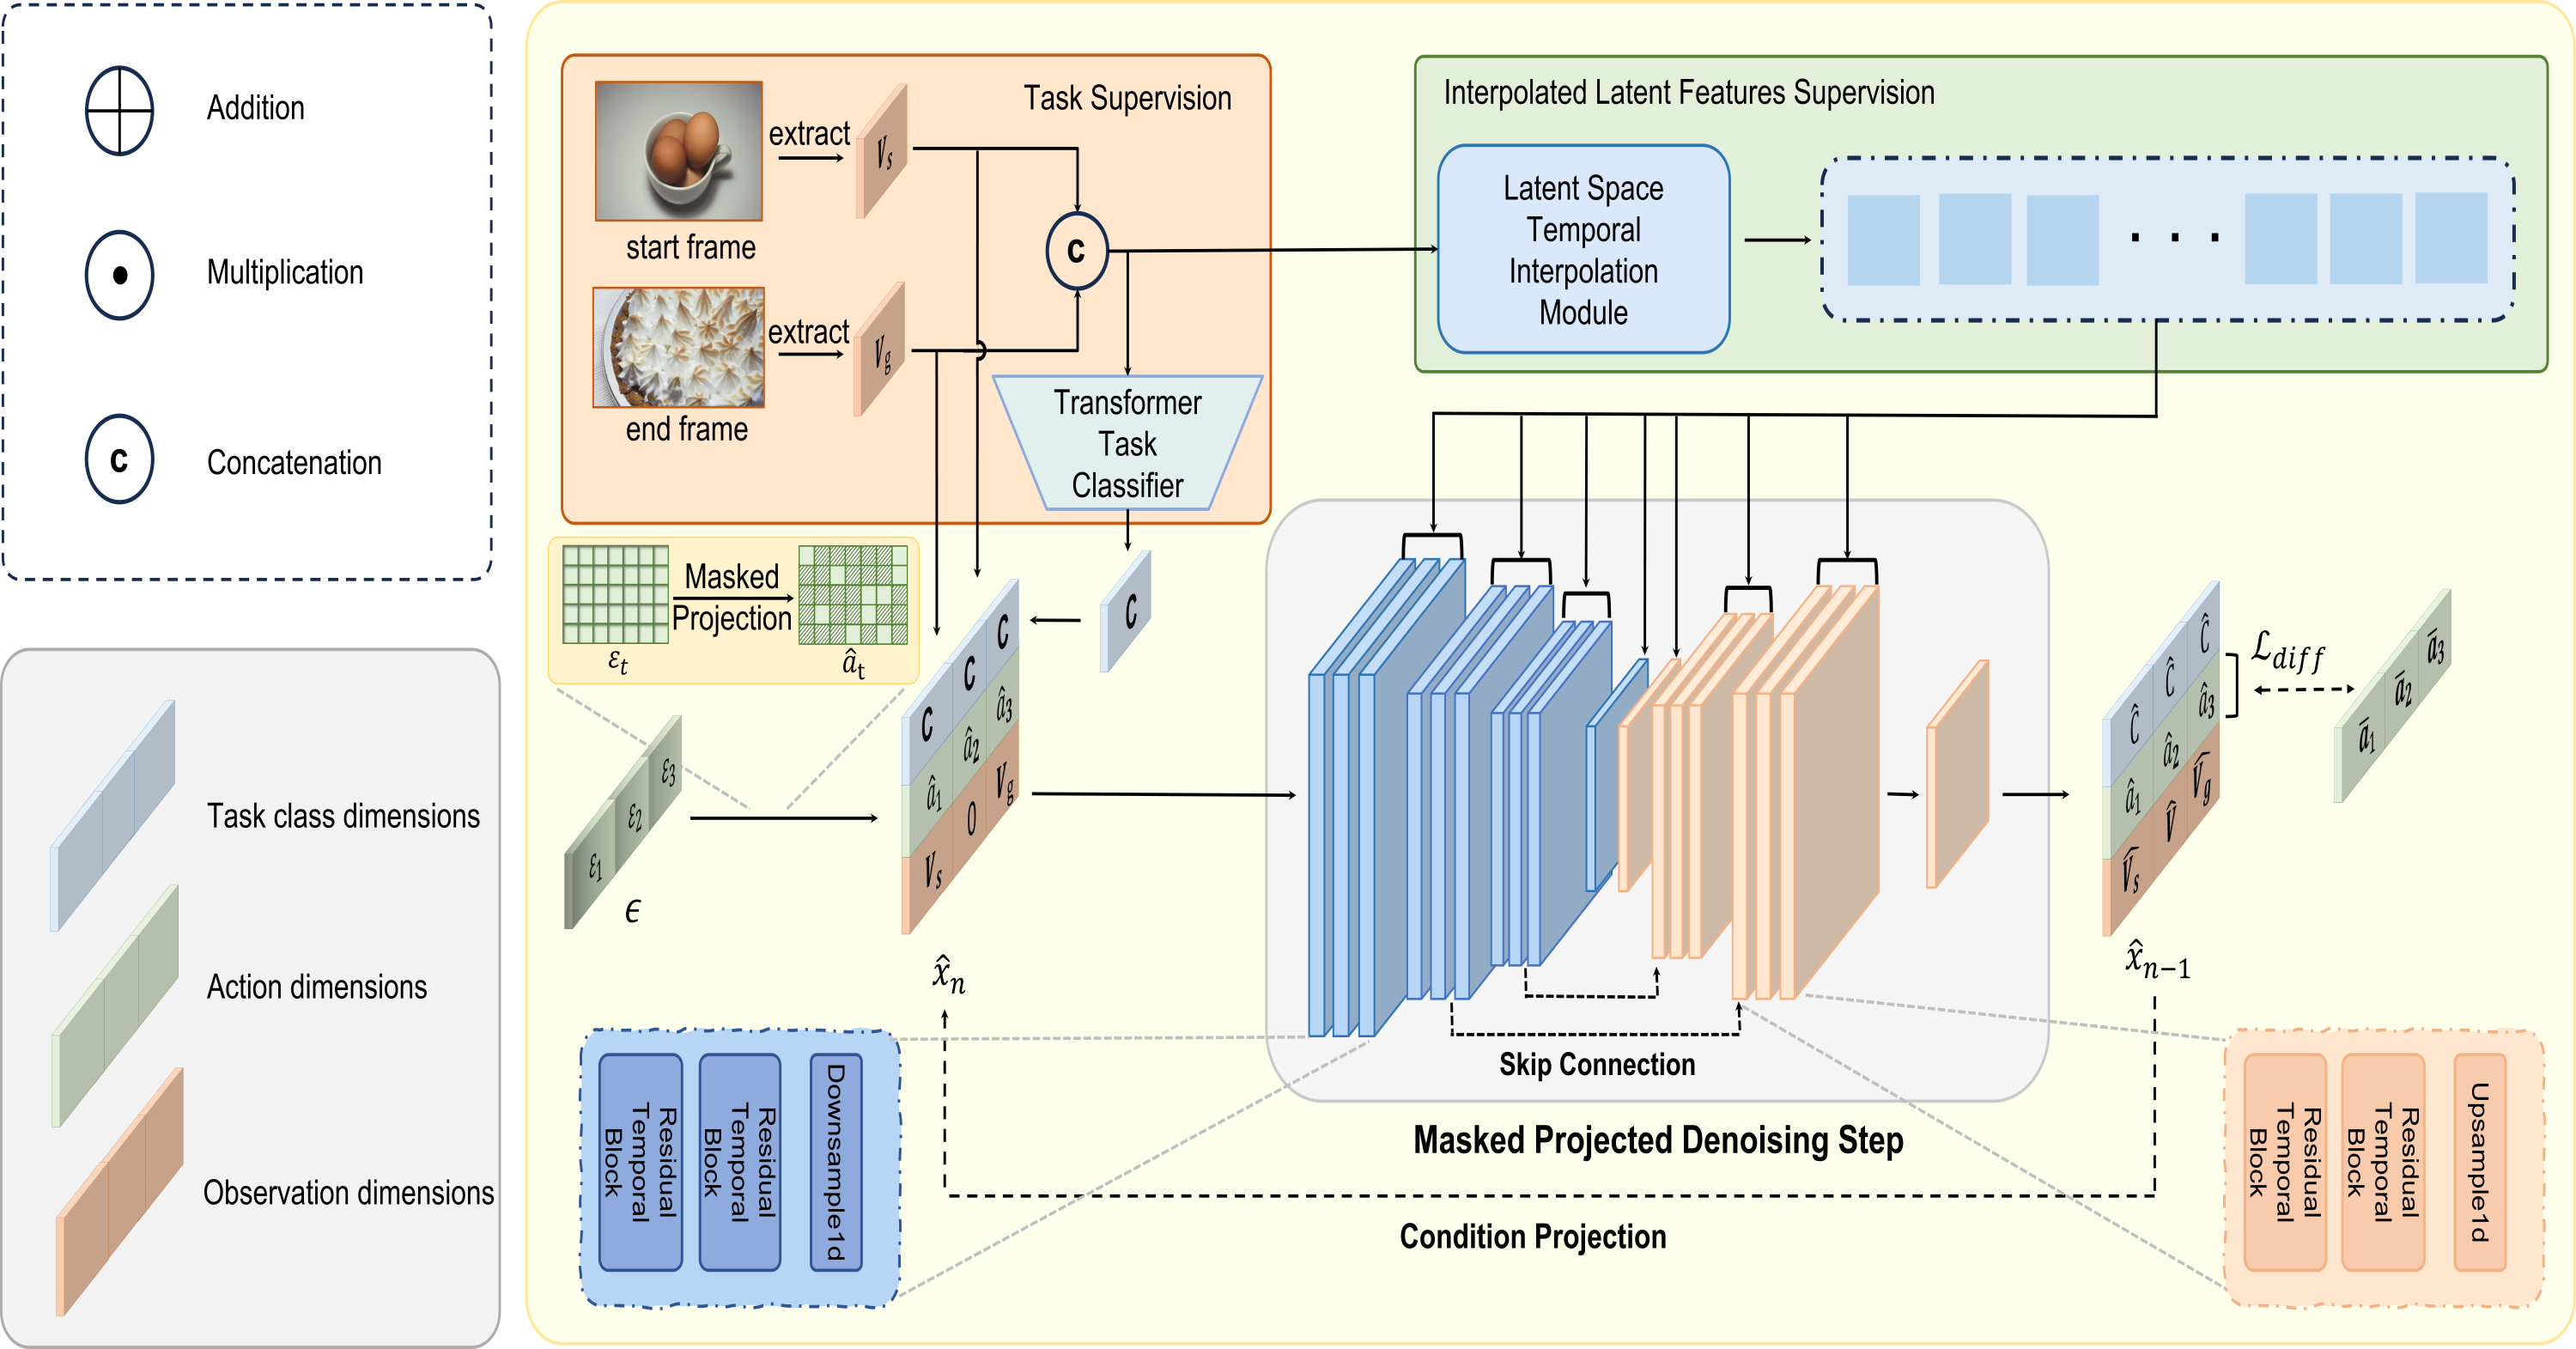
\includegraphics[width=\textwidth,height=0.6\textheight,keepaspectratio]{figures/architecture1.png}
    \caption{Overview of our Masked Temporal Interpolation Diffusion (prediction horizon \( T=3 \)). }
    \label{fig:architecture}
\vspace{-4mm}
\end{figure}
% We first train a transformer task classifier to generate condition information \( c \), which will be used as guidance along with the given observations \( V_s \) and \( V_g \). Subsequently, we put the concatenated observations into the latent space temporal logical interpolation module to obtain the latent temporal logic supervision. Then we compute the denoising process iteratively. In the first step, we conduct a masked projection to the input, then predict the initial distribution by the learned model \( f(\theta) \). We calculate \( \hat{x}_{n-1} \) with the U-Net output \( \hat{x}_0 \). After repeated iterations, we finally select the action dimensions as our result after \( N \) denoising steps.

